\section{POLYFIT Fit Polynomial To Data}

\subsection{Usage}

The \verb|polyfit| routine has the following syntax
\begin{verbatim}
  p = polyfit(x,y,n)
\end{verbatim}
where \verb|x| and \verb|y| are vectors of the same size, and
\verb|n| is the degree of the approximating polynomial.  
The resulting vector \verb|p| forms the coefficients of
the optimal polynomial (in descending degree) that fit
\verb|y| with \verb|x|.  
\subsection{Function Internals}

The \verb|polyfit| routine finds the approximating polynomial
\[
   p(x) = p_1 x^n + p_2 x^{n-1} + \dots + p_n x + p_{n+1}
\]
such that
\[
   \sum_{i} (p(x_i) - y_i)^2
\]
is minimized.  It does so by forming the Vandermonde matrix
and solving the resulting set of equations using the backslash
operator.  Note that the Vandermonde matrix can become poorly
conditioned with large \verb|n| quite rapidly.
\subsection{Example}

A classic example from Edwards and Penny, consider the problem
of approximating a sinusoid with a polynomial.  We start with
a vector of points evenly spaced on the unit interval, along with
a vector of the sine of these points.
\begin{verbatim}
--> x = linspace(0,1,20);
--> y = sin(2*pi*x);
--> plot(x,y,'r-')
\end{verbatim}
The resulting plot is shown here


\centerline{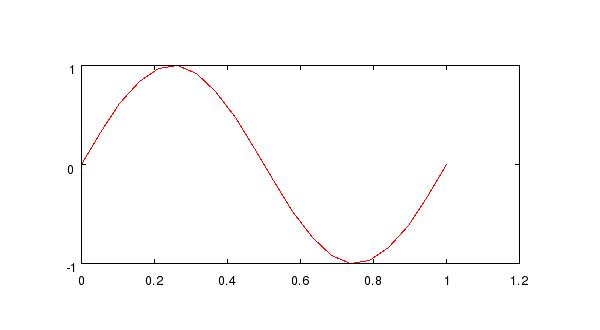
\includegraphics[width=8cm]{polyfit1}}

Next, we fit a third degree polynomial to the sine, and use
\verb|polyval| to plot it
\begin{verbatim}
--> p = polyfit(x,y,3)

p = 
   21.9170  -32.8756   11.1897   -0.1156 

--> f = polyval(p,x);
--> plot(x,y,'r-',x,f,'ko');
\end{verbatim}
The resulting plot is shown here


\centerline{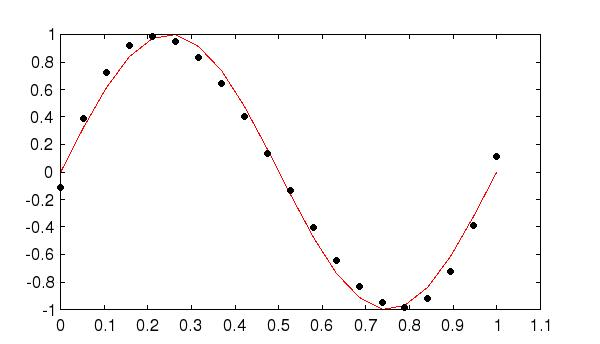
\includegraphics[width=8cm]{polyfit2}}

Increasing the order improves the fit, as
\begin{verbatim}
--> p = polyfit(x,y,11)

p = 

 Columns 1 to 8

   12.4644  -68.5541  130.0555  -71.0940  -38.2814  -14.1222   85.1018   -0.5642 

 Columns 9 to 12

  -41.2861   -0.0029    6.2832   -0.0000 

--> f = polyval(p,x);
--> plot(x,y,'r-',x,f,'ko');
\end{verbatim}
The resulting plot is shown here


\centerline{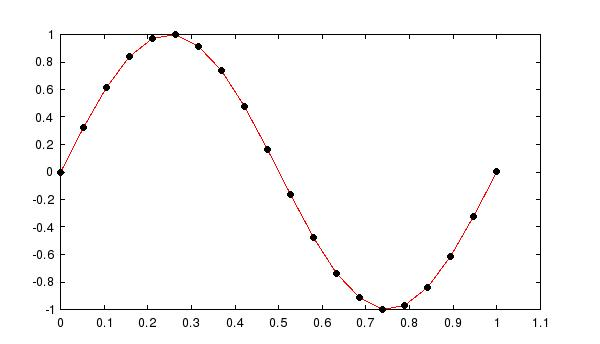
\includegraphics[width=8cm]{polyfit3}}

